% This file was created (at least in part) by the script ParseMdtoLatex by Louis du Plessis
% (Available from https://github.com/taming-the-beast)

\documentclass[11pt]{article}
\input{preamble}

% Add your bibtex library here
\addbibresource{master-refs}


%%%%%%%%%%%%%%%%%%%%
% Do NOT edit this %
%%%%%%%%%%%%%%%%%%%%
\begin{document}
\renewcommand{\headrulewidth}{0.5pt}
\headsep = 20pt
\lhead{ }
\rhead{\textsc {BEAST v2 Tutorial}}
\thispagestyle{plain}


%%%%%%%%%%%%%%%%%%
% Tutorial title %
%%%%%%%%%%%%%%%%%%
\begin{center}

	% Enter the name of your tutorial here
	\textbf{\LARGE Model adequacy using BEAST2}\\\vspace{2mm}

	% Enter a short description of your tutorial here
	\textbf{\textcolor{mycol}{\Large Assessing clock and substitution models}}\\

	\vspace{4mm}

	% Enter the names of all the authors here
	{\Large {\em David Duchêne}}
\end{center}


%%%%%%%%%%%%%%%%%
% Tutorial body %
%%%%%%%%%%%%%%%%%

\section{Background}\label{background}

This tutorial will guide you through methods to assess model adequacy in
BEAST v2.4.x. In common practice, evolutionary models are selected based
on their statistical fit \emph{relative to each other}. This might be
sufficient in some cases, but there is a risk that all of the candidate
models lead to inferences that poorly represent the true evolutionary
process. Indeed, even the most complex or best fitting model from a set
of candidates can produce highly erroneous estimates of parameters of
interest. In this tutorial we will explore methods to investigate the
absolute merits of the model. This kind of assessment of the absolute
performance of models is also known as model checking or assessment of
model adequacy or plausibility.

Before starting the tutorial, it is important that you understand the
methods used in Bayesian inference for assessing model adequacy. A
typical assessment of model adequacy is done by comparing a test
statistic, calculated from the empirical data set, with the values of
the statistic calculated from a large number of data sets simulated
under the model. The simulated data sets from the model are often
referred to as posterior predictive simulations (PPS), and they
represent future or alternative data sets under the candidate model. The
test statistic should be informative about the assumptions of the model
in question.

A large number of test statistics have been proposed to assess the
components of phylogenetic analyses. In this tutorial we will
investigate two test statistics, one for assessing the substitution
model, and one for assessing the priors on rates and times used for
molecular dating (Figure \protect\hyperlink{fig:example1}{1}).

\begin{itemize}

\item
  The multinomial likelihood, which is the likelihood of the data under
  a model with only a single general assumption: that substitution
  events are independent and identically distributed across sites. This
  statistic can be used to assess overall substitution model fit. Note
  that sites with missing data or indels should not be included when
  estimating the multinomial likelihood.
\item
  The $ A $ index assesses the power of the molecular-clock
  model to estimate the number of substitutions across branches,
  assuming a tree topology and an adequate substitution model. We will
  go through this statistic in more detail during this exercise.
\end{itemize}

\section{Programs used in this}\label{programs-used-in-this}

Exercise

\begin{itemize}

\item
  BEAST v2.4.x.
\item
  R programming environment.
\item
  R packages \emph{ape} and \emph{phangorn}. Before starting the
  exercise, install these packages by typing the following in your R
  console:
\end{itemize}

\begin{lstlisting}[language=R]

      install.packages("phangorn")
      
\end{lstlisting}

\clearpage

\section{Run the empirical data}\label{run-the-empirical-data}

The evolutionary history of birds has been widely studied using
mitochondrial DNA. Mitochondrial genomes have been sequenced for a
diversity of birds, including passerines (perching birds). However, can
show substantial differences in nucleotide composition between species.
This potentially violates an assumption that is commonly made in
phylogenetic analyses: that of compositional homogeneity across
lineages.

When we analyse nucleotide sequences, we often compare a number of
substitution models from the GTR family to identify the one that
provides the best fit to our data. However, we typically only consider a
small subset of the models in this family, such as the JC, HKY, and GTR
models. But it is possible that all of the models in this subset
actually provide a poor absolute fit to our data.

Here we investigate whether the widely used GTR+G model of nucleotide
substitution provides an adequate description of the evolutionary
process in mitochondrial DNA from 13 corvid birds (plus an outgroup
taxon). This group of birds includes crows, ravens, and the Eurasian
magpie. The data set comprises 1000 sites from the third codon positions
of mitochondrial protein-coding genes.

In the \lstinline!data! folder you will find the in nexus format
(\lstinline!cp3.nex!) and a previously-estimated topology in newick
format (\lstinline!corvid.tre!) with our corvid taxa. You will also find
an XML file (\lstinline!cp3.xml!) in the \lstinline!xml! folder to run
BEAST 2 for this data set.

The settings in this XML file include:

\begin{itemize}

\item
  A GTR+G substitution model.
\item
  A \textbf{strict clock} with a uniform prior from 0 to 1 (substitution
  per site per million years).
\item
  A Yule tree prior.
\item
  A normally distributed root calibration with standard deviation of 2
  and mean of 40.
\item
  Run length of 10 million steps and the sampling frequency as 1K.
\end{itemize}

Importantly, this XML file has been modified directly such that the
starting tree has been provided and it remains fixed throughout the run.
The steps to modify the XML to fix the tree topology are explained in a
box at the end of this tutorial.

Run the XML file using BEAST 2. The output of this run can also be found
in the folder \lstinline!precooked_runs!.

\section{One step model assessment}\label{one-step-model-assessment}

In this section we will run substitution and clock model assessment. We
will be using the output from the BEAST 2 analysis that we ran in the
previous section. However, \textbf{if you wish to perform model
assessment for your own data, you should follow the steps in this
section.}

The results for the example data set in this section can also be found
in the folder \lstinline!precooked_runs!. In that folder you will also
find the results for the BEAST 2 run of \lstinline!cp3.xml!.

Begin by opening R. By typing the following, you will set the working
directory to the scripts folder, and then load all the necessary scripts
inside it.

\begin{lstlisting}[language=R]

    setwd("INSERT THE PATH TO SCRIPTS FOLDER")
    for(i in dir()) source(i)
\end{lstlisting}

In the next box will set the directory to \lstinline!precooked_runs!,
and run the function \lstinline!adeq()!. The information in quotes in
\lstinline!adeq()! are:

\begin{itemize}

\item
  The path to the posterior of trees from BEAST 2
\item
  The path to the log file from BEAST 2
\item
  The path to the empirical data alignment in nexus format
\end{itemize}

In addition, \lstinline!Nsim = 100! specifies the number of posterior
predictive simulations to be performed.

\begin{lstlisting}[language=R]

    setwd("../precooked_runs")
    clock_adequacy_example <- adeq(trees.file = "cp3.trees", log.file ="cp3.log", empdat.file = "../data/cp3.nex", Nsim = 100)
    names(clock_adequacy_example)
\end{lstlisting}

The contents of \lstinline!clock_adequacy_example! should appear after
the latest line of code. The contents include each of the components
used to assess clock and substitution model adequacy. Elements that have
the word \lstinline!empirical! are test statistics calculated for
empirical data. Elements that say \lstinline!pps! are data for each of
the simulated data sets.

The following are some detailed elements in
\lstinline!clock_adequacy_example!:

\begin{itemize}

\item
  The seventh element \lstinline!empirical_multlik! is the multinomial
  likelihood calculated for the empirical data set.
\item
  The eighth element \lstinline!pps_multliks! are the values of the
  multinomial likelihood calculated for each of the simulated data sets.
\item
  The ninth element \lstinline!mlik_pvalue! is the \emph{P}-value for
  the multinomial likelihood, a proxy for the distance between the
  simulations and the empirical data.
\end{itemize}

The \lstinline!clock_adequacy_example! object should have the same
contents as object
`\lstinline!assessment_provided'' in the file!results.Rdata`:

\begin{lstlisting}[language=R]

    load("results.Rdata")
    names(clock_adequacy_example)
\end{lstlisting}

The following section of this tutorial describes the steps for assessing
model adequacy in more detail.

\section{Steps for assessing model
adequacy}\label{steps-for-assessing-model-adequacy}

\subsection{Reading the runs and simulating
data}\label{reading-the-runs-and-simulating-data}

We will study the code in R and Figure
\protect\hyperlink{fig:example1}{1} in detail. This section is mainly
for reading and discussion, and is aimed for you to cement the steps
required for assessing model adequacy.

Open the \lstinline!adeq.R! file in a text editor of your preference and
you should see the following:

\begin{lstlisting}[language=R]

  adeq <- function(trees.file, log.file, empdat.file, Nsim = 100){
     empdat <- as.phyDat(as.DNAbin(read.nexus.data(empdat.file)))
     seqlen <- ncol(as.matrix(as.DNAbin(empdat)))
     tree.topo <- read.nexus(trees.file)[[1]]
     sims <- make.pps.als(trees.file, log.file, Nsim, seqlen)
     sims <- make.pps.tr(sims, empdat, tree.topo)
     bls <- compile.results(sims)
     return(bls)
 }
\end{lstlisting}

The analysis of empirical data is shown in the blue box in Figure
\protect\hyperlink{fig:example2}{2}. We then need to read the posterior
trees and parameter estimates of the BEAST 2 analysis. The R package
\emph{phangorn} allows us to take these data and run the posterior
predictive simulations, which is shown in the green box in Figure
\protect\hyperlink{fig:example1}{1}. You will find the code to read data
from the posterior and for simulating genetic alignments in
\lstinline!make.pps.als!. This script identifies the model being
assessed and simulates data accordingly. The input required in this step
includes:

\begin{itemize}

\item
  The paths of the posterior files for your analysis.
\item
  The number of simulations you want to perform.
\item
  The sequence length (number of sites in your alignment).
\end{itemize}

If you are interested in how we read and simulate data in R, you can
investigate the \lstinline!make.pps.als! code. The following is the line
in \lstinline!adeq.R! in question:

\begin{lstlisting}[language=R]

    sims <- make.pps.als(trees.file, log.file, Nsim, seqlen)
\end{lstlisting}

If the input file has a greater number of samples than the number of
simulations requested, this will randomly select samples from the
posterior. This is a good moment to discuss or read about how an
alignment can be simulated using parameter estimates from the posterior.

\begin{figure}
    \centering
    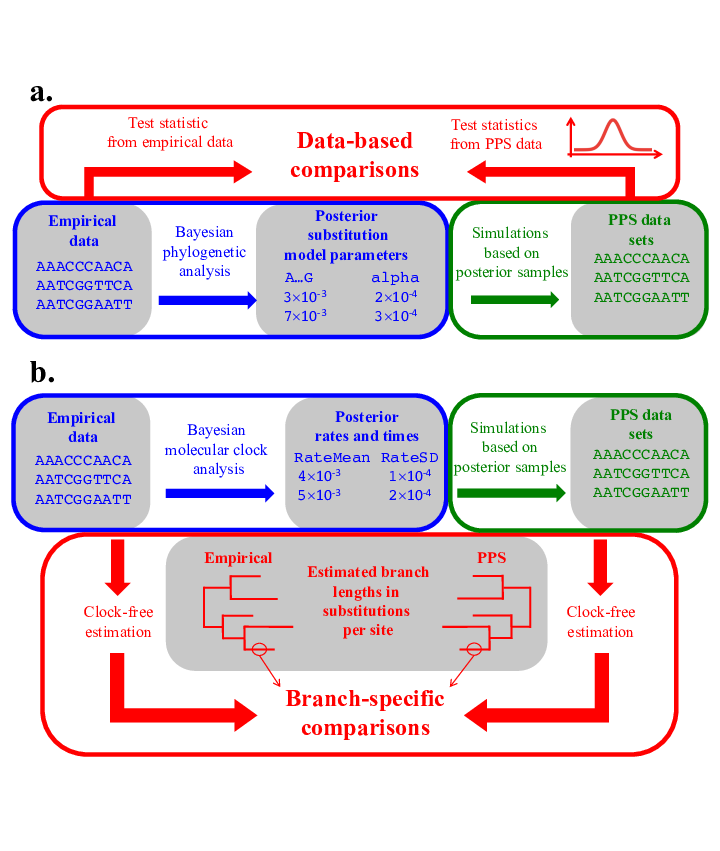
\includegraphics[width=0.800000\textwidth]{figures/Figure_1.pdf}
    \caption{Two of the existing approaches to using posterior predictive simulations to assess model adequacy in Bayesian phylogenetics. (a) One group of methods use characteristics of the data for model assessment, like the multinomial likelihood or the GC content. (b) Another method can assess clock models using estimates from clock-free methods. Under this approach, the number of substitutions per site expected along each branch under the clock hierarchical model are compared with those inferred in a clock-free analysis of the empirical data.}
    \label{fig:example1}
\end{figure}

\clearpage

\subsubsection{Calculate test
statistics}\label{calculate-test-statistics}

Once we have simulated data sets, we can calculate the test statistics.
The function \lstinline!make.pps.trs! takes the assumed tree,
substitution model, and the empirical and simulated data sets. The
function estimates phylogenetic branch lengths for the empirical data
set and each of the simulated data sets. In this step we also estimate
the multinomial likelihood test statistic for the empirical data and
each of the simulated data sets.

\begin{lstlisting}[language=R]

    sims <- make.pps.tr(sims, empdat, tree.topo)
\end{lstlisting}

The output of this function is what we need for model assessment: the
test statistic for the empirical data, and the distribution of test
statistics for the simulated data sets.

\subsubsection{\texorpdfstring{Calculate
\emph{P}-values}{Calculate P-values}}\label{calculate-p-values}

We can now compare the test statistic for the empirical data and each of
the simulated data sets, which is the step shown in the red box in
Figure \protect\hyperlink{fig:example1}{1}. The most common way to do
this is to calculate the tail area probability, which is the number of
simulations with a test statistic greater than the value for the
empirical data.

\begin{lstlisting}[language=R]

    bls <- compile.results(sims)
\end{lstlisting}

This function will provide the test statistics for simulations, as well
as \emph{P}-values for each of the test statistics. Following practice
from frequentist statistics, we can consider the model to be inadequate
if the \emph{P}-value for a given test statistic is below 0.05.
Importantly, the assessment of the clock model allows us to identify the
branches for which the molecular clock model can estimate the number of
substitutions. We will explore the interpretation of these data in the
following section.

\section{Interpreting the results of model
assessment}\label{interpreting-the-results-of-model-assessment}

\subsection{Results of substitution model
assessment}\label{results-of-substitution-model-assessment}

It is strongly recommended to use qualitative checks of models using
graphical analyses. In this section we will graph different components
for assessing clock model adequacy using posterior predictive
simulations.

We will first visualise the results for assessing substitution model
adequacy. The following code makes a histogram of the distribution of
the multinomial likelihood for the PPS data, and will show the position
of the value for empirical data on this distribution.

\begin{lstlisting}[language=R]

    hist(clock_adequacy_example[[8]], 
         xlim = c(min(clock_adequacy_example[[8]])-sd(clock_adequacy_example[[8]]), 
                  max(clock_adequacy_example[[8]])+sd(clock_adequacy_example[[8]])), 
         main = "", xlab = "Multinomial likelihood")

    abline(v = clock_adequacy_example[[7]], col = 2, lwd = 3)
\end{lstlisting}

Your plot will be identical or very similar to Figure
\protect\hyperlink{fig:example2}{2}. When assessing model adequacy, we
consider the model to be an adequate representation of the evolutionary
process if the test statistic for the empirical data is a typical value
arising from the model. The multinomial likelihood for the empirical
data falls inside the distribution of values for simulated data (Figure
\protect\hyperlink{fig:example2}{2}), so our substitution model is
possibly a reasonable description of the process that generated the
data.

This result can also be observed in the \emph{P}-value for the
multinomial likelihood in R:

\begin{lstlisting}[language=R]

    clock_adequacy_example[9]
\end{lstlisting}

\begin{figure}
    \centering
    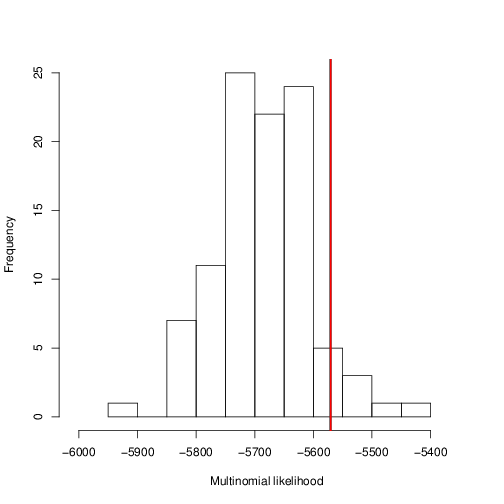
\includegraphics[width=0.700000\textwidth]{figures/Figure_2_multinomial_dist.pdf}
    \caption{Distribution of PPS multinomial likelihood values with the value of the test statistic for the empirical data shown as a vertical line in red.}
    \label{fig:example2}
\end{figure}

\subsubsection{Results of clock model}\label{results-of-clock-model}

assessment

The following script shows a simple example to explore the branch-wise
posterior predictive \emph{P}-values. We will first load the tree. In
this example we will use the original tree provided
(\lstinline!data/corvid.tre!), but usually the tree with the median
posterior branching times would be appropriate. We will colour the
branches with the best accuracy in blue, and the branches that have the
lowest accuracy in green (Figure \protect\hyperlink{fig:example3}{3}).

\begin{lstlisting}[language=R]

   tr <- read.tree("../data/corvid.tre")
   plot(tr, edge.col = rainbow(length(clock_adequacy_example$branch_wise_pppvalues), 
        start = 2/6, end = 4/6)[rank(clock_adequacy_example$branch_wise_pppvalues)], 
        edge.width = 6, cex = 1.5)
   edgelabels(clock_adequacy_example$branch_wise_pppvalues, bg = "white", cex = 1.5, frame = "none")
\end{lstlisting}

The values along each branch indicate the proportion of simulations in
which the branch length was greater than the length estimated using the
empirical data. The expected value under the model is 0.5. If this value
is 0 branch lengths are being underestimated with respect to the model.
Similarly, if the value is 1 branch lengths are being overestimated with
respect to the model.

You can also investigate the $ A $ index:

\begin{lstlisting}[language=R]

   clock_adequacy_example[4]
\end{lstlisting}

This index is the proportion of branches in the tree for which the
branch-wise posterior predictive \emph{P}-values are inside the central
95 percent of the distribution. The rates and times models can be
considered adequate when the $ A $ index is high.

You might find it surprising that the $ A $ index for this
data set is closer to 0 than 1. The reason for this is possibly that we
used an overly simple model of rate variation across lineages. As
described in section 3, the analyses in BEAST 2 were done using a strict
clock. Furthermore, these data have very high overall rates, such that
they have a very large amount of variation, and possibly contain
substantial substitutional saturation.

\begin{figure}
    \centering
    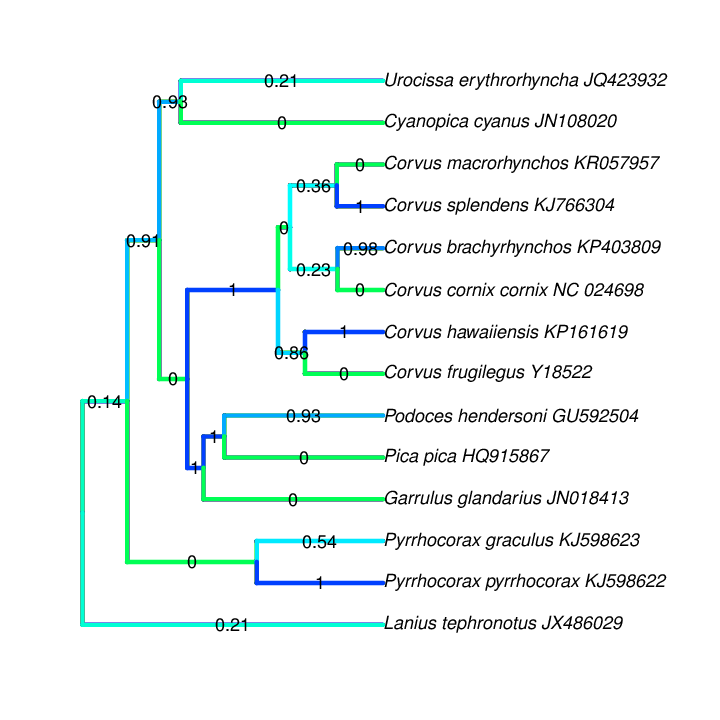
\includegraphics[width=0.900000\textwidth]{figures/Figure_3_branchwise_p.pdf}
    \caption{Estimated chronogram with branches coloured by their clock adequacy P-value.}
    \label{fig:example3}
\end{figure}

\begin{figure}
    \centering
    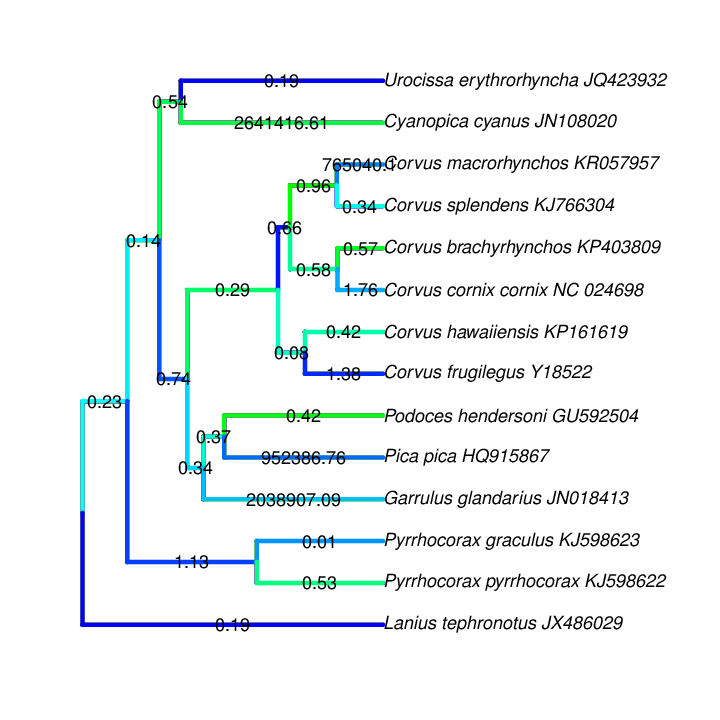
\includegraphics[width=0.900000\textwidth]{figures/Figure_4_branchwise_dev.pdf}
    \caption{Estimated chronogram with branches coloured by their deviation between the empirical and simulated lengths.}
    \label{fig:example4}
\end{figure}

The following script shows a simple example to explore the branch-wise
length deviation. This metric is a proxy for the difference between the
branch-length estimate using empirical data and the mean branch-length
estimate using posterior predictive simulations. To make the values
comparable across branches, the difference between the empirical branch
length and mean PPS branch-length has been divided by the empirical
branch length. If this value is close to zero, the priors for times and
molecular evolutionary rates can be considered adequate. We apply the
same colouring system as the plot above. Note that in the case of branch
length deviation, larger numbers indicate greater deviation from the
empirical branch length, and therefore lower accuracy (Figure
\protect\hyperlink{fig:example4}{4}).

Have a look at the alignment file to observe the large amount of
variation in the data, and why some of the values in Figure
\protect\hyperlink{fig:example4}{4} seem extremely large. One thing you
might notice is that the sites seem highly variable, suggesting that
there might be a large degree of substitutional saturation. Our
conclusion form these analyses is that the strict clock provides a very
poor fit to these data, and a more flexible clock model might be better
suited. In addition, it might be appropriate to use the first and second
codon positions of these mitochondrial genes, because they are likely to
be less saturated.

\begin{lstlisting}[language=R]

    plot(tr, edge.col = rev(rainbow(length(clock_adequacy_example$branch_length_deviation), 
         start = 2/6, end = 4/6)[rank(clock_adequacy_example$branch_length_deviation)]), 
         edge.width = 6, cex = 1.5)
    edgelabels(round(clock_adequacy_example$branch_length_deviation, 2), bg = "white", cex = 1.5, frame = "none")
\end{lstlisting}

Note that in this simple method to graph the results, the branches in
the two plots above have been coloured by their rank, rather than their
magnitude. \clearpage

\section{Concluding remarks}\label{concluding-remarks}

\begin{itemize}

\item
  Assessing model adequacy provides insight into the \emph{absolute}
  merits of a candidate model. This means that it can identify cases
  when even the best-fitting candidate model is a poor representation of
  the evolutionary process, such that inferences are unreliable.
  Assessment of model adequacy is an alternative to traditional model
  selection approaches that assess the \emph{relative} support among
  candidate models.
\item
  The choice of test statistic is critical to the assessment of model
  adequacy. The test statistic can define what aspect of a model is
  being assessed. Most test statistics are not complete descriptions of
  the model, so it is convenient to explore a model using several test
  statistics where possible.
\item
  There are cases in which the inferences of some parameters are
  reliable, while others are not (e.g.~some branch rates are accurate
  while others are not). Closer examination of test statistics can
  sometimes bring additional insight into when the model is adequate for
  the data at hand.
\end{itemize}

\clearpage

\begin{framed}
\textbf{Optional: Fixing the tree topology}

Load the data \lstinline!cp3.nex! to BEAUti, setting the model as
described in the first section, and saving the XML file. Then open the
XML file in your preferred text editor, and add a \lstinline!tree!
statement as follows above line with the \lstinline!<run ...! statement.

\begin{lstlisting}[language=XML]

    <tree id="Tree.t:treename" spec='beast.util.TreeParser' newick="((A, B), (C, D), E);" taxa="@alignmentname"/>
\end{lstlisting}

Newick refers to a format to express the tree structure. Replace the
dummy newick tree with the correct tree, which you will find in
\lstinline!corvid.tre! in the \lstinline!data! folder. Also modify the
names of the tree and the taxa: the name of your tree appears after
\lstinline!"Tree.t:! elsewhere in the XML, and the name of the taxa is
an \lstinline!@! followed by your data \lstinline!id! in the line
immediately above the alignment.

Now remove the \lstinline!tree! statement, which is inside the
\lstinline!state! and looks like the following.

\begin{lstlisting}[language=XML]

    <tree id="Tree.t:treename" name="stateNode">
            <taxonset id="TaxonSet.alignmentname" spec="TaxonSet">
                <alignment idref="alignmentname"/>
            </taxonset>
     </tree>
\end{lstlisting}

In the place of that \lstinline!tree! statement, type an
\lstinline!input! statement, which will lead to a new
\lstinline!statenode! as follows.

\begin{lstlisting}[language=XML]

    <input name='stateNode' idref='Tree.t:treename'/>
\end{lstlisting}

Once again, make sure that the tree name is correct.

Now remove the whole random tree initialiser, which begins and ends with
the following lines.

\begin{lstlisting}[language=XML]

    <init id="RandomTree.t:treename" ...
    ...
    </init>
\end{lstlisting}

Lastly, remove the lines (or set the weights to 0) of the operators on
the tree topology. These include the lines that have any of
\lstinline!SubtreeSlide!, \lstinline!Narrow!, \lstinline!Wide!, and
\lstinline!WilsonBalding!. You might find these words together with the
tree model selected (in this case \lstinline!BirthDeath!).
\end{framed}

\clearpage



%%%%%%%%%%%%%%%%%%%%%%%
% Tutorial disclaimer %
%%%%%%%%%%%%%%%%%%%%%%%
% Please do not change the license
% Add the author names and relevant links
% Add any other aknowledgments here
\href{http://creativecommons.org/licenses/by/4.0/}{\includegraphics[scale=0.8]{figures/ccby.pdf}} This tutorial was written by David Duchêne for \href{https://taming-the-beast.github.io}{Taming the BEAST} and is licensed under a \href{http://creativecommons.org/licenses/by/4.0/}{Creative Commons Attribution 4.0 International License}. 


%%%%%%%%%%%%%%%%%%%%
% Do NOT edit this %
%%%%%%%%%%%%%%%%%%%%
Version dated: \today



\newpage

%%%%%%%%%%%%%%%%
%  REFERENCES  %
%%%%%%%%%%%%%%%%

\nocite{*} 

\printbibliography[heading=relevref]


\end{document}